% might need psfig, url, amsmath, amsfonts?
\documentclass[psfig]{acm_proc_article-sp}

\begin{document}

\title{StreamIt: A Compiler for Streaming Applications}

\numberofauthors{1}
\author{
\alignauthor \vspace{-18pt} Saman Amarasinghe, Matthew Brown, Michael Gordon, Henry Hoffmann, Michal Karczmarek, David Maze, Bill Thies, and Jeremy Wong\\
	\vspace{12pt}
	Laboratory for Computer Science \\
	Massachusetts Institute of Technology \\
	Cambridge, MA  02139 \\
	\vspace{12pt}
	{\tt \{saman, morris, mgordon, hank, karczma, dmaze, thies, jnwong\}@lcs.mit.edu} \\
	\vspace{12pt}
        \today
}

% for the arrow of a function def, etc.
\newcommand{\ma}[2]{max_{#1 \rightarrow #2}}
\newcommand{\mi}[2]{min_{#1 \leftarrow #2}}
\newcommand{\floor}[2]{\left\lfloor\frac{#1}{#2}\right\rfloor}
\newcommand{\ceil}[2]{\left\lceil\frac{#1}{#2}\right\rceil}
\newtheorem{definition}{Definition}

\maketitle

\begin{abstract}
%Due to the high data rates involved in audio, video, and signal
processing applications, it is imperative to compress the data to
decrease the amount of storage used.  Unfortunately, this implies that
any program operating on the data needs to be wrapped by a
decompression and re-compression stage.  Re-compression can incur
significant computational overhead, while decompression swamps the
application with the original volume of data.

In this paper, we present a program transformation that greatly
accelerates the processing of compressible data.  Given a program that
operates on uncompressed data, we output an equivalent program that
operates directly on the compressed format.  Our transformation
applies to stream programs, a restricted but useful class of
applications with regular communication and computation patterns.  Our
formulation is based on LZ77, a lossless compression algorithm
utilized by ZIP, and immediately applies to simpler formats such as
Apple Animation, Microsoft RLE, and Targa.

We implemented a simple subset of our techniques in the StreamIt
compiler, which emits executable plugins for two popular video editing
tools: MEncoder and Blender.  For common operations such as color
adjustment and video compositing, computing directly on compressed
data offers a speedup roughly proportional to the overall compression
ratio.  For our benchmark suite of 12 videos in Apple Animation
format, speedups range from 1.1x to 471x, with a median of 15x.

\end{abstract}

%\section{Introduction}


Stream computing represents an increasingly important class of
applications. In streaming codes, there is an abundance of parallelism that
is easier to extract compared to traditional desktop workloads (e.g.,
pointer-based computing). As a result, the extraction of parallelism
in streaming codes does not require heroic efforts, and thus,
processors can deliver higher performance with significantly lower
power costs. This is especially important since
leading microprocessor companies have realized that modern general
purpose architectures are near their  performance limits for  the
amount of power they consume. Thus, the future will place a greater
emphasis on exploiting the properties of streaming workloads in
conventional von~Neumann architectures.

Streaming is a model of computation that uses sequences of data
and computation kernels to expose concurrency and locality for
efficiency~\cite{wss}. In general purpose processors, improving locality 
translates to an effective management of the memory hierarchy at all
levels, including the register file. In this paper, we present a
methodology for compiling streaming codes to general purpose,
cache-based architectures. We first introduce a simple model for
reasoning effectively about the caching behavior of streaming
workloads. This model serves as a foundation for several {\it cache-aware
optimizations} that are geared toward the concomitant increase of instruction
and data {\it temporal locality}. These
optimization lead to significantly better utilization of the memory
system, and as such, they deliver performance gains ranging from 11
to 99\% for our streaming benchmark suite.

The context for our work is StreamIt, an architecture-independent
language that is engineered for streaming
applications~\cite{streamitcc}. It adopts the 
Cyclo-Static Dataflow~\cite{BELP96} model of computation which is a
generalization of Synchronous Dataflow~\cite{LM87-i} (SDF).  
SDF is a popular  model that  is well suited for
streaming codes. In SDF, computation is represented as a graph
consisting of {\it  actors} connected by communication channels; the
actors consume  and produce a constant number  of items from their
input and output  channels every time they execute. SDF is appealing
because it is amenable to static scheduling and optimization. 

From a general purpose architecture's point of view, actors represent
computation kernels, and the communication between actors represents
data buffers that must be streamed to and from the processor. Thus
the size of an actor and the
order of actor executions are critical properties that
impact the performance of the instruction cache. For example, the
compiler must make sure the actor's code size is not
greater than the instruction cache. Furthermore, we must {\it scale}
the execution of the actor so that it runs several times before we move
on to some other actor in the stream 
graph. This serves to $(i)$ amortize the cost of fetching the actor's
instructions into the cache from memory (an expensive operation), $(ii)$
improve the instruction temporal locality, and $(iii)$ improve overall
performance. However, as our cache model will show, we 
cannot arbitrarily scale the execution frequency of an actor. This
is because actors produce data that must be buffered, and therefore,
we must also consider the amount of data an actor produces and
consumes if we are to adequately manage the data cache. This paper is unique
in that it is the first to present a unified optimization methodology
that simultaneously considers instruction and data locality for
mapping streaming computation to cache-based architectures.

In terms of improving the data cache behavior, the compiler schedules
actor firing such that the producer-consumer locality is
preserved. Furthermore,  the compiler may {\it fuse}
together two or more actors to form a coarser grained kernel.
The fusion allows for better register allocation as we can
destroy the arrays used to buffer data between the actors and replace
the corresponding array references with scalars.  It also allows for
various competing implementations for managing the buffers between the
fused actors.  This paper evaluates several implementation
alternatives (for buffer management) and evaluates their performance.

The methodology for fusing actors leverages a distinguishing StreamIt
characteristic, namely, the hierarchical organization of
the stream graph. Furthermore, the algorithm for fusing actors applies
for the various topologies allowed by StreamIt.
It also considers another distinguishing characteristics of StreamIt,
namely the {\tt peek} operation whereby an actor may inspect data
items in its input buffer without consuming them until some future
execution. While peeking is a powerful language feature, it does pose
some challenges to the compiler and the cache optimizations. Peeking
also impacts the choice for the best buffer management strategy, as our
study will show.

%% the comment about p3 and itanium not being embedded architectures
%% is out of the blue! need a better transition.
Cache-aware fusion alone delivers significant performance gains, although our
evaluation shows that fusion with scaling leads to the best
performance on a general purpose, cache-based architecture. For our
experiments, we use two different processors: a superscalar out-of-order
processor, and an in-order VLIW processor. The former is a Pentium~3
whereas the latter is an Itanium~2. While these architectures are not
particularly suited for an embedded system, they do exhibit some
properties that are worthy of investigation. Furthermore, that we can
demonstrate measurable performance gains on real systems is far more
convincing than using a simulation-based environment. We chose the
Pentium~3 processor because it has very few registers in its
instruction set architecture. The Itanium by contrast has a much 
larger and richer repertoire of registers. The two architectures serve
to validate our cache-aware optimizations, in that we expect an
architecture with more register to benefit more from optimization such
as scalar replacement. On average, fusion leads to a 47\% improvement
on the Pentium~3, and 50\% on the Itanium~2.

The two architectures also differ in terms of their memory system
organization. The Itanium is an in-order VLIW processor and does not
tolerate a memory stall as well as its out-of-order
counterpart. Therefore we expect different gains from the scaling
optimization which amortize the long access latencies for instruction
and data caches. On average, scaling leads to a 21\% improvement on
the Itanium~2, and 17\% on the Pentium~3.

While both scaling and fusion lead to modest performance gains, we
must combine the two to deliver the best possible performance. When we
do so, we can further improve the performance of our benchmarks by
53\% on average for the Pentium~3, and 55\% for the Itanium~2.

\subsection{Summary of Contributions}

This paper makes the following contributions:
\begin{itemize}

\item A cache model for stream computing that provides a quantitative
estimate of the caching performance for any sequence of actor
executions.

\item A cache-aware scheduling heuristic that judiciously increases
the multiplicity of actors, improving instruction and data locality
while not exceeding the data cache.

\item A cache-aware partitioning policy that judiciously fuses
adjacent actors into a single component, enabling local optimizations
while not exceeding the instruction cache.

\item An optimized buffer management policy, termed ``copy-shift with
execution scaling'', which out-performs a traditional rotating buffer
in a detailed micro-benchmark analysis.

\item A fully automatic implementation of the above techniques in the
StreamIt compiler.

\item An experimental evaluation across 11 streaming benchmarks,
demonstrating performance improvements of up to 99\%.
\end{itemize}

\subsection{Paper Roadmap}

The remainder of the paper is organized as follows. Section~\ref{sec:streamit}
describes StreamIt and introduces our motivating example.
Section~\ref{sec:cache-model} introduces our cache model for 
reasoning about the performance of a streaming
computation. Section~\ref{sec:cache-opt} describes our cache-aware
optimizations, and Section~\ref{sec:buffer} describes the 
optimization enabled by fusion. Section~\ref{sec:evaluation} describes
our evaluation methodology and present our experimental
analysis. Sections~\ref{sec:related-work}~and~\ref{sec:conclusion}
discuss related work and concludes the paper.

%\section{StreamIt}
\label{sec:streamit}

StreamIt  is   an  architecture-independent  language that was
designed for  streaming applications. In StreamIt, programs are
represented as graphs where  nodes represent  computation and edges
represent FIFO-ordered communication of data over tapes.

The  basic programmable  unit (i.e., an actor) in  StreamIt is a {\it
filter}.   Each filter contains  a work  function that executes
atomically,  popping (i.e., reading)  a fixed number  of items  from
the  filter's input  tape and pushing (i.e., writing) a fixed number
of items to the filter's output tape.  A filter  may also {\tt peek} at
a given index  on its input tape without  consuming  the  item;  this
makes  it  simple  to  represent computation over a
sliding-window.   The {\tt push}, {\tt pop}, and {\tt peek} rates are
declared as part  of  the work  function,  thereby enabling  the
compiler    to construct a static schedule of filter executions. The
following is an example implementation of a FIR   (Finite Impulse
Response)  filter: 
%\begin{scriptsize}
{\small
\begin{verbatim}
float->float filter FIR (int N, float[] weights) 
{
  work push 1 pop 1 peek N {
    float sum = 0;
    for (int i = 0; i < N; i++) {
      sum += peek(i) * weights[i];
    }
    pop();
    push(sum);
  }
}
\end{verbatim}}
%\end{scriptsize}

The work function is invoked (fired) whenever there is sufficient data
on the input tape. In this case, the filter requires at least
\texttt{N} elements before it can execute. The value of \texttt{N} is
known at compile time when the filter is composed to form a stream
graph. A filter is akin to a class in object oriented programming
with the work function serving as the main method. The parameters
to a filter (e.g., \texttt{N} and \texttt{weights}) are equivalent to
parameters passed to a class constructor. In StreamIt, the
application developer focuses on the hierarchical assembly of the
stream graph and its communication topology, rather than on the 
explicit management of the data buffers between filters.

\begin{figure}[t]
\begin{center}
\vspace{-24pt}
 \framebox{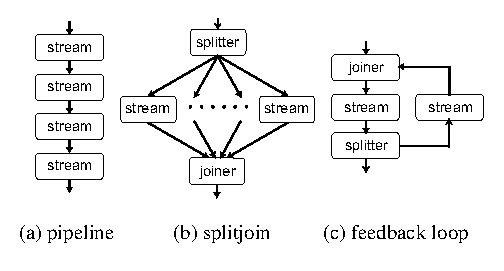
\includegraphics[scale=1, angle=0]{./constructs-eg.eps}}
 \vspace{-6pt}
 \caption{StreamIt containers.}
 \label{fig:containers}
\end{center}
\end{figure}

\begin{figure}[t]
\begin{center}
\vspace{-12pt}
 \framebox{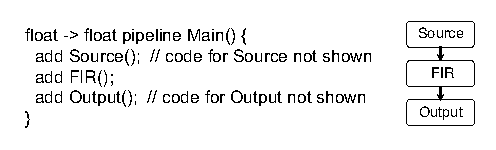
\includegraphics[scale=1, angle=0]{./pipeline-eg.eps}}
 \vspace{-6pt}
 \caption{Example pipeline with FIR filter.}
 \label{fig:pipeline}
\vspace{-18pt}
\end{center}
\end{figure}

StreamIt provides three hierarchical structures for composing filters
into larger stream graphs (see Figure~\ref{fig:containers}). The 
{\it pipeline} construct composes streams in sequence, with the output
of one connected to the input of the next.   An example of a pipeline
appears in Figure~\ref{fig:pipeline}.

The {\it splitjoin} construct distributes data to a set of parallel
streams, which are then joined together in a round robin fashion.  In
a splitjoin, the {\it splitter} performs the data scattering, and the
{\it joiner} performs the gathering. A splitter is a specialized
filter with a single input and  multiple output channels. On 
every execution step, it can distribute its output to any one of
its children in either a {\it duplicate} or a {\it roundrobin}
manner. For the former, incoming data is replicated to every
sibling connected to the splitter. For the latter, data is scattered
in a round-robin manner, with each item sent to exactly one child
stream, in order.  The splitter type and the weights for distributing data to
child streams are declared as part of the syntax (e.g., \texttt{split
duplicate} or \texttt{split roundrobin($w_0$, $w_1$, ... $w_n$)}). The
splitter counterpart, the joiner, is a specialized filter with  
multiple input channels but only one output channel. The joiner
gathers data from its predecessors in a round-robin manner (declared
as part of the syntax). 

StreamIt also provides a {\it feedback loop} construct for introducing
cycles in the graph.

\section{Execution Model}
\label{sec:execmodel}

A StreamIt program is represented by a hierarchical graph,
where the leaf nodes are filters, splitters, and joiners, and
the composite nodes are pipelines, splitjoins, and
feedback-loops. Edges in the graph represent data channels, which 
operate as FIFO queues.
In order for an actor  (i.e., a filter,
splitter, or joiner) to execute, it must have enough data items on its input
tape. In StreamIt, actors have  two epochs
of execution: one for initialization, and one for the steady
state. The initialization primes the input tapes to allow filters with
peeking to execute the very first instance of their work functions;
initialization in this setting is similar to the prologue stage in
software pipelining. The steady state schedule has the property that
the amount of data buffered between any two actors does not change
before and after the actor executions.

\begin{figure}[t]
\begin{center}
\vspace{-24pt}
 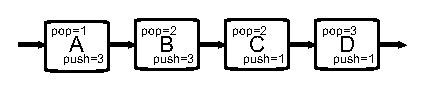
\includegraphics[scale=1, angle=0]{./pipe-with-rates.eps}
\vspace{-6pt}
 \caption{Example pipeline.}
 \label{fig:pipe-with-rates}
\end{center}
\end{figure}

As an example, a steady state schedule for the sample pipeline in
Figure~\ref{fig:pipe-with-rates} requires filter \texttt{A} to fire
four times, \texttt{B} six times, \texttt{C} nine times, and
\texttt{D} three times. 
% Because in StreamIt the filters are
% independent (i.e., they do not share state), they can execute
% concurently. In a uniprocessor setting (which is what we use for our
% evaluation), we can only run one filter at time. Therefore, 
The data generated by one actor is buffered (cached) until it is
consumed.

The StreamIt compiler derives the initialization and steady state
schedules~\cite{karczma-lctes03} and outputs a C program that includes
the initialization and work functions, as well as a driver to execute
each of the two schedules. For example, referring to
Figure~\ref{fig:pipe-with-rates}, the compiler generates the following
sample code for running the steady state schedule:
%\begin{scriptsize}
\begin{verbatim}
run_steady_state() {
  for (i = 0; i < 4; i++) A_work();
  for (i = 0; i < 6; i++) B_work();
  for (i = 0; i < 9; i++) C_work();
  for (i = 0; i < 3; i++) D_work();
}
\end{verbatim}
%\end{scriptsize}
To execute the program, the steady state kernel is wrapped with
another loop that invokes the kernel a designated number of
times. Preceding the state steady, a similar initialization schedule
is run to prime the data buffers, and following the steady state, an
epilogue is run to drain the buffers as necessary.

\begin{figure}[t]
\begin{center}
\vspace{-12pt}
 \psfig{figure=ssi.eps,width=3in}
 \vspace{-6pt}
 \caption{Instruction size (in bytes along the y-axis) per filter
 (x-axis) occurring in a steady state execution of FFT.}
 \label{fig:ssi-single}
\vspace{-18pt}
\end{center}
\end{figure}

From a caching point of view, it is intuitively clear that once a
filter's instruction working set is fetched into the cache, we must
execute that filter as many times as possible to improve instruction
locality and amortize the cost of the accesses to lower levels of the
memory hierarchy. This of course assumes that the total code size for
the filters in the steady state exceeds the capacity of the
instruction cache (which is commonly the case;). In
Figure~\ref{fig:ssi-single} we show a representative breakdown of the
code size per filter in a steady state execution of a StreamIt
implementation of FFT. In all, the total code size for a steady state
ranges from 16~Kb to over 60~Kb for our benchmarks. These results
provide evidence that while individual filters may have a
small instruction footprint, the total footprint of the filters in a
steady state exceeds a typical instruction cache size.
From these observations, it is evident that we must {\it scale} the
execution of filters in the steady state in order to improve temporal
locality. In other words, rather than running a filter $S$ times per
steady state, we increase the loop bound so that it runs $\texttt{M}
\times S$ times (e.g., the loop bound for \verb+A_work+ is
changed to $\texttt{M} \times 4$ in the example shown earlier). 
We term \texttt{M} the {\it multiplicity factor}.

The obvious question is: to what extent can we scale the execution of
filters in the steady state? The answer is non-trivial because
scaling, while beneficial to the instruction cache behavior, may
overburden the data cache as the buffers between actors may grow to
prohibitively large sizes that degrade the data cache
behavior. Specifically, if a buffer overflows the cache, then
produce-consumer locality is lost. 

Also complicating matters is the amount of state a filter must retain
from one execution of its work function to the next. In the FIR
example shown earlier, the filter state is proportional to the size of
the coefficient array (i.e., \texttt{weights}). The filter state
further constrains the schedule scaling.

%% \begin{figure}
%% \centering
%% \psfig{figure=tapes.eps,width=2.5in}
%% \caption{A filter's input and output tapes during an execution step.
%% With each step, the filter pushes two items, pops two items, and peeks
%% at three additional items.  The initial state of the input tape is
%% shown at left.  The center shows the filter with both input and output
%% tapes during the invocation of {\tt work}.  The final state of the
%% output tape is shown at right.}
%% \label{fig:tapes}
%% \end{figure}

\begin{figure}
\centering
\psfig{figure=pipeline.eps,width=1.76in}

(a) A Pipeline. \\
\vspace{8pt}
\psfig{figure=splitjoin.eps,width=3.0in}

(b) A SplitJoin. \\
\vspace{8pt}
\psfig{figure=feedback.eps,width=2.33in}

(c) A FeedbackLoop. \\
\caption{StreamIt structures with labeling.}
\vspace{-12pt}
\label{fig:tapelabels}
\end{figure}

\section{Streaming Model of Computation}

In this section, we develop an abstract model of streaming computation
to serve as a basis for reasoning about program transformations and
compilation techniques within the streaming domain.  A stream graph
differs from a traditional, sequential program in that all of the
filters of the graph are implicitly running in parallel, with the
execution order constrained only by the availability of data on
channels between the filters.  Further, filters communicate only with
their immediate neighbors, thereby removing any notion of global time
or non-local dependences of one filter on another.  [add idea that it
is the specification of the atomic work function that really prevents
global time] These properties merit the development of a new model of
computation, in which the notions of timing, scheduling, and
dependence analysis are in terms that are relative to a given filter
in the graph, instead of being global characteristics of a program.

In Section \ref{sec:minfunc}, we develop a transfer function that
provides the basis for distributed time in a stream graph... [build
operational semantics to give a precise meaning to messaging, and
denotational semantics to validate program transformations].

\subsection{Notation}

We use the following notation:

\begin{itemize}

\item A {\it tape} is an infinite history of the values that have been
  pushed onto a channel between two filters. We use $I_S$ and $O_S$ to
  denote the input and output tapes of stream $S$, respectively, with
  numbering used to distinguish between multiple input or output tapes
  (see Figure \ref{fig:tapelabels}).  Finally, $n(T)$ represents the
  number of items on tape $T$ at a given point of execution.  [should
  we define $p(T)$ here or wait until we use it?  long time def-use!]

\item We say that a filter $A$ is {\it upstream} of filter $B$ (or,
  equivalently, $B$ is {\it downstream} $A$) if there is a directed
  path in the stream graph from $O_A$ to $I_B$.  We use this
  terminology for tapes as well as filters.

\item The number of items that are pushed, popped, and peeked by
  filter $A$ during a single execution of its work function are
  denoted by $push_A$, $pop_A$, and $peek_A$, respectively.  Note that
  $peek_A$ includes the items that are popped, such that $pop_A \le
  peek_A$.

\end{itemize}

\subsection{Relative Time}
\label{sec:minfunc}

As outlined above, there is no concept of global time in a stream
graph since each filter is completely independent and can only
communicate with its neighbors through input and output channels.
Thus, if two filters need to synchronize an event, the synchronization
must be in terms of the data items that are passed over a channel.

In this context, we define a $min$ function between tapes in the
stream graph that allows disconnected filters to have a common notion
of time.  The function is defined in terms of data dependence:
\begin{definition}
$\mi{a}{b}(x)$ is the minimum number of items that must appear on tape
$a$ given that there are $x$ items on tape $b$.
\end{definition}
We now turn to deriving $\mi{a}{b}$ for all pairs of tapes $a$ and $b$
in a filter graph where $a$ is upstream of $b$.

\subsubsection{Filters}

Let us derive $\mi{I_A}{O_A}(x)$, which represents the time shift
across a single filter $A$.  Since the filter produces $push_A$ items
on every invocation, it must be invoked
$\left\lceil\frac{x}{push_A}\right\rceil$ to produce the $x$'th item.
On each invocation, it consumes $pop_A$ items, and peeks at an
additional $peek_A-pop_A$ items.  Thus, the total number of items that
must be present on the input is:
\begin{align}
\label{eq:minfilter}
\mi{I_A}{O_A}(x) = \left\lceil\frac{x}{push_A}\right\rceil*pop_A+(peek_A-pop_A)
\end{align}

\subsubsection{Pipelines}
\label{sec:timepipe}

Let us now derive an expression for $min$ in the case of a pipeline.
In the base case, consider that two filters are connected, with the
output of $A$ feeding into the input of $B$ (see
Figure~\ref{fig:tapelabels}).  We are seeking $\mi{I_A}{O_B}(x)$: the
minimum number of items that must appear on tape $I_A$ given that
there are $x$ items on tape $O_B$.  Observing that a minimum of
$\mi{I_B}{O_B}(x)$ items must appear on tape $I_B$, and that $I_B$
must equal $O_A$ since the filters are connected, we see that a
minimum of $(\mi{I_A}{O_A} \circ \ma{I_B}{O_B})(x)$ items must appear
on $I_A$:
\begin{align*}
\mi{I_A}{O_B} = \mi{I_A}{O_A} \circ \mi{I_B}{O_B}
\end{align*}
By identical reasoning, this composition law holds for pipelined
streams as well as filters.  That is, a Pipeline of streams $S1 \dots
Sn$ has the following $min$ function:
\begin{align}
\label{eq:composepipe}
\mi{S1}{Sn} &= \mi{I_{S1}}{O_{S1}} \circ \dots \circ \mi{I_{Sn}}{O_{Sn}}
\end{align}
One might be tempted to define the $min$ function for any pair of
connected tapes as the composition of functions for the operators
connecting those tapes.  However, such a definition turns out to be
problematic for the SplitJoin and FeedbackLoop constructs, which
require a slightly different composition law for their components (as
shown below).  Instead, we can further extend our notation to include
the {\it components} of streams that are connected in a pipeline.
That is, if tapes $t_i$ and $t_j$ are contained within stream
constructs $S_i$ and $S_j$, respectively, and $S_i$ and $S_j$ belong
to a pipeline of streams $S_1 \dots S_n$, then:
\begin{align}
\label{eq:composetape}
\mi{t_i}{t_j} &= \mi{t_i}{O_{S_i}} \circ \mi{I_{S_{i+1}}}{O_{S_{i+1}}}
\circ \dots \circ \mi{I_{S_j}}{t_j}
\end{align}

\subsubsection{SplitJoins}
\label{sec:timesj}

We now derive $min$ expressions for the components of a SplitJoin, and
for the SplitJoin construct as a whole.  We denote the $n$ output
tapes of the splitter $S$ by $O1_S \dots On_S$, and the $n$ input
tapes of the joiner $J$ by $I1_J \dots In_J$ (see Figure
\ref{fig:tapelabels}).

{\bf Duplicate splitter.}  We consider the $i$'th output tape of an
$n$-way duplicating splitter.  Since the splitter duplicates each
input item onto each output tape, there must be at least $x$ items on
$I_S$ if there are $x$ items on $Oi_S$.  This yields a simple
expression for $min$:
\begin{align*}
\mi{I_S}{Oi_S}(x) = x
\end{align*}

{\bf Weighted round robin splitter.}  Let us consider an $n$-way
splitter with weights $w_1 \dots w_n$.  Observe that if there are
$n(On_S)$ items on the $n$'th output tape, then the splitter must have
executed $\floor{n(On_S)}{w_n}$ complete cycles in distributing items
to the output tapes; each cycle draws $sum_{i}{w_i}$ items from the
input tape $I_S$.  Further, if there are $n(Oi_S)$ items on the $i$'th
output tape, then $n(Oi_S) mod w_i$ additional items have been
deposited on $Oi_S$ during the current cycle of the splitter, and
$n(Oi_S)~mod~w_i + sum_{j=0}^{i-1}{w_j}$ items have been drawn from
the input since the last complete cycle.  Summing the item count for
the completed cycles and the current cycle gives the following
expression for $min$:
\begin{align*}
\mi{I_S}{Oi_S}(x) = \floor{n(On_S)}{w_n} * \sum_{i}{w_i} + x~mod~w_i +
\sum_{j=0}^{i-1}{w_j}
\end{align*}

{\bf Weighted round robin joiner.}  The reasoning is similar for an
$n$-way joiner with weights $w_1 \dots w_n$.  Let us use $W$ to denote
the sum of the weights: $W = \sum{i=1}^{n}{w_i}$.  If there are $x$
items on the output tape $O_J$, then the joiner must have executed
$\floor{x}{W}$ complete cycles, each of which drew $w_i$ items from
the $i$'th input tape.  Since the last complete cycle, the joiner has
drawn $x~mod~W$ items from its inputs, and $MIN(0, x~mod~W -
\sum_{j=0}^{i-1}{w_j})$ of these items were taken from input tape $j$.
Thus, the $min$ function from the output of the joiner to the $i$'th
input tape is as follows:
\begin{align*}
\mi{Ii_J}{O_J}(x) = w_i * W + MIN(0, x~mod~W - \sum_{j=0}^{i-1}{w_j})
\end{align*}

{\bf SplitJoin construct.}  As with the Pipeline construct, we can
derive the $min$ function across an entire SplitJoin as a composition
of the component functions.  However, a SplitJoin differs from a
Pipeline in that the joiner imposes a control dependence between the
parallel streams.  That is, for there to be $x$ items on the output of
the joiner, there must be at least $\mi{Ii_J}{O_J}(x)$ items on {\it
every} input tape $Ii_J$.  Applying the composition law for pipelines
(Equation \ref{eq:composepipe}), it follows that there must be at
least at least $\mi{Oi_S}{Ii_J} \circ \mi{Ii_J}{O_J}(x)$ items on
every output tape $Oi_S$ of the splitter.  Finally, the minimum number
of items appearing on the input tape $I_S$ of the splitter is the {\it
maximum} of the item requirement from any output tape $Oi_S$.  By this
reasoning, the $min$ function for a SplitJoin is as follows:
\begin{align}
\mi{I_S}{O_J}(x) &= MAX_{i \in [1,n]}(\mi{I_S}{Oi_S} \circ
\mi{Oi_S}{Ii_J} \circ \mi{Ii_J}{O_J})(x)
\end{align}

\subsubsection{FeedbackLoops}
\label{sec:timefl}

The $min$ function for a feedback loop requires extra care. Although
the feedback splitter $FS$ serves as a normal splitter, with the same
$min$ function as derived above, the feedback joiner $FJ$ is slightly
different due to the initialization phase of the loop.  Also, the
$min$ function does not compose across all components of the loop,
since otherwise there would be conflicting definitions for paths that
circle the loop several times.

{\bf Feedback joiner}.  For a feedback loop with delay $d$, the
feedback joiner must fabricate its first $d$ input values, since no
items have yet been pushed onto the loop tape $I2_{FJ}$.  This means
that there must be an offset of $d$ in the $min$ function, since the
first $d$ items are direct inputs to the joiner instead of appearing
as items on the input tape.  Using $J$ to denote a weighted round
robin joiner as considered above, we thus have the following
expression for the $min$ function across the feedback path:
\begin{align*}
\mi{I2_{FJ}}{O_{FJ}}(x) = \mi{I2_J}{O_J}(x) - d
\end{align*}
However, the $min$ function remains unchanged with respect to the
input from the main stream:
\begin{align*}
\mi{I1_{FJ}}{O_{FJ}}(x) = \mi{I1_J}{O_J}(x)
\end{align*}

{\bf Feedback components}.  Within a feedback loop, the $min$ function
between tape $a$ and any downstream tape $b$ can be uniquely defined
by composing the $min$ functions along the directed acyclic path
between $a$ and $b$.  We require an acyclic path to avoid successive
passes around the loop, which would prevent a unique definition of the
function.  Denoting this path of tapes by $(a, t_1, \dots , t_n, b)$,
the composition follows the form of Equation \ref{eq:composepipe}:
\begin{align*}
\mi{a}{b}(x) = \mi{a}{t_1} \circ \mi{t_1}{t_2} \circ \dots \mi{t_n}{b}
\end{align*}
Note that these functions can then be composed with those of
constructs neighboring the feedback loop to obtain, for instance, the
relation between the loop tape $I2_{FJ}$ and a downstream pipeline (by
application of Equation \ref{eq:composetape}).

{\bf Feedback loop construct.}  As a special case of the equation
above, we can see that the $min$ function for the feedback loop as a
whole is the composition of the $min$ functions along the main path:
\begin{align*}
\mi{I1_{FJ}}{O_{FS}}(x) = \mi{I1_J}{O_J}(x) \circ \mi{I1_J}{O_J}(x) 
\end{align*}
Intuitively, this is because--in any semantically correct stream
program--the loop itself is guaranteed to have enough inputs to feed
the joiner, such that the output tape of the feedback loop places a
restriction only on the input tape of the feedback loop.

\subsubsection{Summary}

In the preceding sections, we have derived a $min$ function for the
components of each stream construct, as well as for the stream
construct as a whole.  By application of Equation
\ref{eq:composetape}, this yields a function $\mi{a}{b}$ for every
pair of tapes $a$ and $b$ where $b$ is downstream of $a$.

[say some more profound stuff about the min function?  information
  flow, NOT data dependence.  The data dependence is in the work
  functions themselves; this is a property of the graphs.  distributed
  time.]

\subsection{Program Verification}
\label{sec:prog-verif}

A number of program analysis techniques are immediately afforded by
the $min$ function.  In particular, it is very simple to compute 1)
whether or not the program will deadlock as a result of a starved
input channel, and 2) whether or not any buffer will grow without
bound during the steady-state execution of the program.

{\bf Deadlock detection.}  The deadlock detection algorithm takes
advantage of the fact that the only loops in our stream graph are part
of a FeedbackLoop construct.  A stream graph will be deadlock-free if
and only if every feedback loop produces enough data to satisfy its
own feedback joiner.  This can be formulated in terms of the $min$
function by considering $min_{t}{t}$, the data that a tape $t$ in a
feedback loop requires of itself.  However, since we didn't define
$min$ across circular paths in the stream graph, we will denote this
function by $minloop$ and define it at the loop input to the feedback
joiner:
\begin{align*}
minloop(x) \equiv \mi{I2_{FJ}}{O_{FJ}} \circ \mi{O_{FJ}}{I2_{FJ}}
\end{align*}
Now, the loop will be deadlock-free if and only if $\forall x \in N, x
- minloop(x) > 0$.  This condition follows directly from
causality--the $x$'th item can be produced if and only if its
production depends only on some subset of the $x-1$ items that are
already on the channel.

{\bf Overflow detection.}  There are two places that a buffer can grow
to an unbounded size in the stream graph.  The first is in a feedback
loop, when\footnote{$f(x) = \omega(g(x))$ if $lim_{x \rightarrow
\infty}\frac{f(x)}{g(x)} = \infty$}~$x - minloop(x) = \omega(1)$.
That is, if $minloop(x)$ items on the feedback tape enables the
production of an additional $x - minloop(x)$ items that grows
asymptotically with the position $x$ on the tape, then the constant
consumption rate will not keep up with the growing production rate,
and the buffer will overflow.

The second case of buffer overflow is when the parallel streams of a
SplitJoin have asymptotically different production rates.  For a given
stream $i$ in a SplitJoin construct, the buffer corresponding to the
joiner input tape $Ii_J$ will overflow if and only if there is a
stream $j$ in the SplitJoin for which:
\begin{align*}
(\mi{I_S}{Oi_S}& \circ \mi{Oi_S}{Ii_J} \circ \mi{Ii_J}{O_J})(x) - \\
(\mi{I_S}{Oj_S}& \circ \mi{Oj_S}{Ij_J} \circ \mi{Ij_J}{O_J})(x) = \omega(1)
\end{align*}
Both of these cases could be detected by a compiler to verify that no
buffers will overflow during steady-state execution.

\subsection{Information Flow}

In the above sections, the $min$ function is mostly described in terms
of data dependences.  However, we can also think of this function as
defining a common timing mechanism that asynchronous filters can use
to synchronize events.  We present this timing mechanism in terms of
``information flow'', which we believe is a central concept of the
streaming domain.  Using this concept, we give a precise semantics to
message delivery timing in in StreamIt.

\subsubsection{Information Wavefronts}

When an item enters a stream, it carries with it some new information.
As execution progresses, this information cascades through the stream,
effecting the state of filters and the values of new data items which
are produced.  We refer to an ``information wavefront'' as the set of
filter executions that first sees the effects of a given input item.
Thus, although each filter's {\tt work} function is invoked
asynchronously without any notion of global time, two invocations of a
work function occur at the same ``information-relative time'' if they
operate on the same information wavefront.

The $min$ function can be used to give a precise definition to an
information wavefront.  One interpretation of $y = \mi{a}{b}(x)$ is
that the item at position $y$ of tape $a$ is the the latest item on
tape $a$ to {\it effect} the item at position $x$ of tape $b$.  This
is because item $x$ on tabe $b$ can be produced if and only if tape
$a$ contains at least $y$ items.  Note that this effect might be via a
control dependence rather than a data dependence--for instance, if
item $y$ needs to pass through a round-robin joiner before some data
from another stream can be routed to tape $b$.  This is why we choose
``information flow'' instead of ``data flow'' to describe the timing
concept.  Also, when speaking of the information wavefront, we only
consider information that is passed through the data streams; if a
data item effects another via a low-latency downstream message, then
this effect could jump ahead of the wavefront.

\subsubsection{Message Timing}
\label{sec:messagesemantics}

We now employ the $min$ function to give a precise meaning to the
message delivery guarantees in StreamIt.  Suppose that filter $A$
sends a message to filter $B$ with latency $\lambda$, where $\lambda$
is any integer.  After $\lambda$ invocations of $A$'s {\tt work}
function, $A$ will produce (or has produced) one or more data items
$d$.  Now, the messaging system guarantees that:
\begin{enumerate}

\item If $B$ is upstream of $A$, then $B$ will receive the message
immediately following the last invocation of its {\tt work} function
which produces items that affect $d$.

\item If $B$ is downstream of $A$, then $B$ will receive the message
immediately preceding the first invocation of its {\tt work} function
which produces items that are effected by $d$.

\end{enumerate}
Now let us express these constraints in terms of the $min$ function.
Letting $s$ be equal to $n(O_A)$ at the time that the message was
sent, we have that:
\begin{enumerate}

\item If $B$ is upstream of $A$, the message will be delivered when:
\begin{align}
\label{eq:msgup}
n(O_B) = push_B * \ceil{\mi{O_B}{O_A}(s + push_A * \lambda)}{push_B}
\end{align}
That is, $s + push_A * \lambda$ is the number of items on $A$'s output
tape after producing the data of interest.  Then, $y = \mi{O_B}{O_A}(s
+ push_A * \lambda)$ is the latest item on $B$'s output tape that
affects the data of interest.  The message should be delivered
immediately after the work function producing this item, which occurs
when the item count $n(O_B)$ equals $push_B * \ceil{y}{push_B}$, as
specified by the constraint.

\item If $B$ is downstream of $A$, the message will be delivered when:
\begin{align}
\label{eq:msgdown}
n(O_B) = MAX(x~s.t.~\mi{O_A}{O_B}(x) = s + push_A * (\lambda-1))
\end{align}
That is, $z = s + push_A * (\lambda - 1)$ is the number of items on
$A$'s output tape before pushing the data of interest.  The message
should be delivered when $B$ has executed as far as possible given
that there are $z$ items on $O_A$.  That is, $B$ should push $x$ items
on its output tape for the maximum $x$ that still depends on some of
the $z$ items, which is given by the condition $\mi{O_A}{O_B}(x) = z$
above.

Thus, when $A$ pushes the next set of data, it could affect the data
that will be pushed next onto the output tape of $B$.  (Note that the
next set of data from $A$ might not be sufficient to calculate the
next set on $B$'s output, but it could affect it nonetheless.)  The
message must be delivered immediately before this effected data
appears on $B$'s output, so the number of items $n(O_B)$ is as given
above.  We do not need a ceiling function as in (1) because we are
guaranteed to have the maximum $x$ at a multiple of $push_B$.

\end{enumerate}

\subsubsection{Latency Constraints}

The framework describe above can be used to give a semantics to the
latency constraints in StreamIt.  Each directive MAX\_LATENCY(A, B, n)
has the same effect as defining a message from filter $B$ to upstream
filter $A$ with latency $n$.

\subsection{Operational Semantics}

We can fully define the possible sequences of filter executions as a
set of constraints on the number of items on each tape in the stream
graph.  This is useful not only from the perspective of semantics, but
for compiler analysis of the space of valid schedules.  To begin the
analysis, we formulate the constraints imposed by message delivery
guarantees on the number of items on each tape.

Suppose that a filter $A$ might send a message to filter $B$ with a
maximum latency of $\lambda$ during any invocation of its work
function.  Then we must constrain the execution of $B$ to make sure
that it is not too far ahead to receive the message with the given
latency.  That is, we can only execute $B$ so long as $n(O_B)$--the
item count on its output tape--does not exceed the count when a
message would be delivered.  Recalling the expression for message
delivery time (Equations \ref{eq:msgup} and \ref{eq:msgdown}), this
constraint is as follows if $B$ is upstream of $A$:
\begin{align}
\label{eq:mc1}
n(O_B) \le push_B * \ceil{\mi{O_B}{O_A}(n(O_A) + push_A * \lambda)}{push_B}
\end{align}
and as follows if $B$ is downstream of $A$:
\begin{align}
\label{eq:mc2}
n(O_B) \le MAX(x~s.t.~\mi{O_A}{O_B}(x) = n(O_A) + push_A * (\lambda-1))
\end{align}
The guarantees for latency are treated identically to message
guarantees, as fitting with the semantics of latency as described
above.

{\bf Defining the schedule.}  We now have a set of constraints
expressing whether or not a given set of tapes respects the latency
and message delivery guarantees in a program.  We will now
incorporate these constraints into an operational semantics that
defines a legal sequences of filter executions.

We represent a stream graph as a configuration $(\langle p(t_1),
n(t_1) \rangle,$ $\langle p(t_2), n(t_2) \rangle,$ $\dots,$ $\langle
p(t_k), n(t_k) \rangle)$, where $t_1 \dots t_k$ are the tapes in the
stream graph, and $p(t)$ represents the number of items that have been
popped from tape $t$.  Obviously, we have the constraint that $p(t)
\le n(t)$ for each tape $t$, since a filter can only pop as many items
as have appeared on its input tape.

When the program begins, no items have been pushed or popped from any
data channels.  Thus, each tape is empty, and the starting
configuration $C_0$ is simply the zero vector.  It is possible that
the initial configuration violates some of the constraints imposed by
the messaging and latency constructs, in which case the compiler can
inform the programmer that the delivery constraints requested in the
program are unsatisfiable.

Let ${\cal P}(C)$ denote whether or not the constraints in
Equations~\ref{eq:mc1} and~\ref{eq:mc2} are satisfied for all filters
in a stream graph with configuration $C$.  We can then write the
transition function between configurations as follows:
\[
\begin{scriptsize}
\begin{array}{c}
n(I_A) - p(I_A) \ge peek_A; \\ (\dots , \langle p(I_A), n(I_A) \rangle, \dots,
\langle p(O_A), n(O_A) \rangle, \dots); \\ {\cal P}((\dots , \langle p(I_A)+pop_A, n(I_A) \rangle, \dots,
\langle p(O_A), n(O_A)+push_A \rangle, \dots)); \\ \hline (\dots , \langle p(I_A)+pop_A,
n(I_A) \rangle, \dots, \langle p(O_A), n(O_A)+push_A \rangle, \dots)
\end{array}
\end{scriptsize}
\]
There are two components of this rule.  On the first line, we state
that, for filter $A$ to fire, there must be at least $peek_A$ items on
$A$'s input tape that have not yet been popped.  Secondly, we express
that once $A$ has fired, the new configuration must satisfy the
messaging and latency constraints ${\cal P}$.  The new configuration differs
from the original only in that $pop_A$ items have been popped from
$A$'s input and $push_A$ items have been pushed to $A$'s output.

\subsection{Denotational Semantics}

The operational semantics above defines the space of legal execution
orderings for the filters in a stream graph, but says nothing about
the values that are being pushed onto the tapes.  For this we develop
a denotational semantics, with which we can prove that certain
transformations preserve the meaning of the entire program.

Our denotational semantics contains three algebras: one for literal
StreamIt syntax, one for an intermediate abstract syntax, and one for
the semantic analysis.  The purpose of the intermediate algebra is to
provide a simplified syntax for developing stream transformations, and
to abstract away the StreamIt-specific aspects of the program.  We
provide an informal description of how to translate back and forth
between StreamIt programs and the abstract syntax, and then consider
more formal valuation functions for determining the meaning of the
abstract syntax within the semantic algebra.  Throughout the analysis,
we assume that filters are stateless and that the stream program is
semantically correct.

\subsubsection{Intermediate Algebra}
\label{sec:intalgebra}

The intermediate algebra provides a common mathematical representation
for manipulating stream programs.  Though we have referred to this
algebra as providing an abstract syntax for stream programs, the
representation is strictly a mathematical framework within semantic
domains rather than a program that is fit for execution.  Nonetheless,
the LISP-like syntax allows us to think of the representation as a
program that is amenable to straightforward transformation techniques.

\begin{figure}
\begin{align*}
&Item = Real \\
i~\in~&Index = N \\
g~\in~&IndexTransform = Index \ra Index \\
t~\in~&Tape = Index \ra Item \\
&Pop, Peek, Push = N \\ 
f~\in~&WorkStatement = IndexTransform \ra (Tape \ra Item) \\ 
&WorkFunction = WorkStatement^{+} \\
S~\in~&SplitType = \{Duplicate, WeightedRR\} \\ 
J~\in~&JoinType = \{WeightedRR\}
\end{align*}
\vspace{-18pt}
\caption{Semantic domains that are shared between the intermediate and
  transform algebras.
\protect\label{fig:shareddom}}
\vspace{-6pt}
\begin{align*}
s~\in~&Stream = Filter + Pipeline + SplitJoin + FeedbackLoop \\
&Filter = Push \times Pop \times Peek \times WorkFunction \\
&Pipeline = Stream^{+} \\
&SplitJoin = SplitType \times Stream^{+} \times JoinType \\
&InitFeedback = Int^{+} \\
&BodyStream, LoopStream = Stream \\
&FeedbackLoop = JoinType \times BodyStream \times \\
& \hspace{0.5in} LoopStream \times SplitType \times InitFeedback
\end{align*}
\vspace{-18pt}
\caption{Semantic domains specific to the intermediate algebra.
\protect\label{fig:interdom}}
\vspace{-6pt}
\begin{align*}
&StreamTransform =  IndexTransform \ra (Tape \ra Tape)
\end{align*}
\caption{Semantic domains specific to the transform algebra.
\protect\label{fig:transformdom}}
\end{figure}

The domains of the intermediate algebra are shown in
Figures~\ref{fig:shareddom}~and~\ref{fig:interdom}.  The algebra
represents tapes as an infinite mapping from an index to an item.
Generally, stream constructs are represented as a list of their
component streams, and filters' work functions are encoded as a list of
push statements that--given the transform from their local indexing to
the global tape position--returns a mapping from a tape to an output
item.

{\bf Converting to the intermediate algebra}.  It is straightforward
to generate an expression in the intermediate algebra that reflects
the meaning of a given StreamIt program.  Due to space limitations, we
consider here only the translation of the work functions.

The translation of a filter's work function contains two steps.  First,
the function is arranged in a {\it canonical form}, in which each pushed
item is given as a direct function of the peeked items, and all of the
pop statements are at the end of the function.  For example: \\
\vspace{0.2in}
\begin{scriptsize}
\begin{tabular}{l}
{\tt void work()}\{ \\
\hspace{12pt} {\tt output.push(} $f_1$ {\tt (input.peek(0), ... , input.peek(PEEK-1) )} \\
\hspace{12pt} $\dots$ \\
\hspace{12pt} {\tt output.push(} $f_{PUSH}$ {\tt (input.peek(0), ... , input.peek(PEEK-1) )} \\
\hspace{12pt} {\tt for (int i=0; i$<$POP; i++) \{ input.pop(); \}} \\
\}
\vspace{-12pt}
\end{tabular}
\end{scriptsize}
Above, we model the computation of the work function as pure
mathematical functions that can be injected into the semantic domain.
The algebraic work function, then, is the alternate application of each
push statement's function $f$, with the index expressions transformed
from their local index $x$ to a global index $g(x)$ on the input tape.
\begin{align*}
{\cal W}&[{\tt void~work() \{...\}}]: {\tt StreamIt Work} \ra
WorkFunction = \\
(&g \ra (t \ra f_1(t(g(0)), \dots , t(g(PEEK-1)))), \\
\dots \\
&g \ra (t \ra f_{PUSH}(t(g(0)), \dots , t(g(PEEK-1)))))
\end{align*}

{\bf Converting from the intermediate algebra}.  To convert back to
StreamIt, we can perform the inverse of the translation shown above,
with a push statement for each function and a local index expression $x$
in place of the global index $g(x)$.  Common sub-expression elimination
can be used to eliminate duplicate peek statements or shared portions of
the $f_i$'s.

\subsubsection{Transform Algebra}

The transform algebra is designed to express the meaning of a stream
graph as a transformation from an input tape to an output tape.  Its
semantic domains are given in Figures \ref{fig:interdom} and
\ref{fig:transformdom}.  We now give the valuation function ${\cal S}:
Stream \ra StreamTransform$ for converting from the intermediate
algebra to the transform algebra.  For a filter, we have:
\begin{align*}
&{\cal S} [(Filter~push~pop~peek~(f_1~\dots~f_{push}))] = g \ra (t \ra
(i \ra \\ &(f_{i~\%~push})(i_{local} \ra g(\mi{I_F}{O_F}(i) - peek + 1 + 
i_{local}))(t))
\end{align*}
That is, the value that a filter pushes onto the $i$'th position of its
output tape is calculated with its function at index $if~\%~push$.  By
the definition of $min$, the index offset to the last value the filter
peeks is $\mi{I_F}{O_F}(i)$, where $I_F$ and $O_F$ denote the input and
output tapes of the filter (as shown in Equation \ref{eq:minfilter},
this is a pure function of $push$, $pop$, and $peek$).  Thus, the offset
to the first value the filter peeks is $\mi{I_F}{O_F}(i) - peek + 1$,
and we obtain the global index by adding this offset to the local index
$i_{local}$.

For a pipeline, the transform function is simply the composition of the
transforms of component streams.  At the internal connections of the
pipeline, the index transform is the identity function, but at the start
of the pipeline we apply the transform $g$ to interface the pipeline to
its outside connection.
\begin{align*}
{\cal S} [(Pipeline~s_1~s_2~\dots~s_n)] = \\
g \ra ({\cal S}[s_n]({\cal I}) \circ \dots \circ {\cal S}[s_2]({\cal I}) \circ {\cal S}[s_1](g)) \\
where~{\cal I}~denotes~the~identity~function
\end{align*}
The valuation function for a SplitJoin follows the same idea, but the
notation is slightly heavier.  Given that we have a round robin joiner
with weights $w_1 \dots w_n$ and $W = \sum{w}$, we first represent the
parallel stream $p(i)$ which computes the $i$'th output of the
joiner:
\begin{align}
\label{eq:p}
p(i) = MIN(j~s.t.~\sum_{k=0}^{j-1}{w_i} \le i~mod~W)
\end{align}
Now, the $i$'th tape position assumes the value that is produced along
stream $p(i)$ in the SplitJoin, and the value of interest appears at
position $\mi{Ip(i)_J}{O_J}(i)$ on the output tape of stream $p(i)$.
The indexing function transforms the stream's local index $i_{local}$
for its own input tape to the corresponding index
$\mi{I_S}{Op(i)_S}(i_{local})$ for the input tape of the splitter:
\begin{align*}
&{\cal S} [(SplitJoin~S~s_1~s_2~\dots~s_n~J)] = g \ra (t \ra (i \ra \\
&(({\cal S}[s_{p(i)}])(i_{local} \ra
g(\mi{I_S}{Op(i)_S}(i_{local}))))(\mi{Ip(i)_J}{O_J}(i))))
\end{align*}
This completes the formulation of the transform algebra.  Using this
algebra, we can express the meaning of any StreamIt program as a
mathematical transformation between infinite tapes.  We will utilize
this formulation to prove that certain transformations of the stream
graph preserve the meaning of the program.

%% $\cal{S}$ 
%%   [(FeedbackLoop (. S) $s_body$ $s_loop$ (. J) ($init_1 \dots
%%   init_n$))] = ??????

\section{Scheduling}

\begin{figure}
\centering
\psfig{figure=sched_diag.eps,width=3.0in}
\caption{The three different scheduling schemes.}
\label{fig:sched}

\end{figure}

Scheduling the order of the execution of filters has a large impact on 
the behavior of a StreamIt program.  In this section we introduce three
different scheduling techniques and analyze their properties.

\subsection{Periodic Schedule}
A schedule for a StreamIt program needs to satisfy a requirement that
a repeated execution of the schedule cannot lead to changed data
buffering between filters.  We call a schedule that satisfies this
requirement a periodic schedule.  (Here a schedule represents the
multiplicity of executions of filters, ignoring the ordering of these
executions.)

For every valid program, there exists a unique, minimal periodic
schedule.  Every other periodic schedule for a StreamIt program is a
multiple of the underlying periodic schedule \cite{bhat1994x3}.

While computing periodic schedules for StreamIt, we chose to preserve the
hierarchical structure presented in the program.

A filter has a periodic schedule of a single execution.  This is
because there are no scheduler-visible buffers inside of a filter.
All other components of the program express their periodic schedules
in terms of number of executions of their subcomponents necessary to
construct a valid schedule.  This technique relies on Theorem {\bf
???} to assure that the periodic schedule built is indeed the minimal
periodic schedule.

\subsection{Initialization Schedule}

Before we can execute any periodic schedule on a program, the program
may require intialization.  This is because we allow filters with
$peek_A$ values greater than their $pop_A$ values.  If the program is
not initialized, a filter that peeks more than it pops would not be
able to consume all the input provided for it during the first
execution of a periodic schedule.  The subsequent executions would
force the filter to consume the exact same amount of data, eventually
causing buffer overflow.

The initialization schedule is computed by ensuring that every filter $A$ has
at least $peek_A - pop_A$ unread data on its input tape available after 
initialization has been completed.

\subsection{Single Appearance Schedule}

A single appearance schedule (SAS) is a schedule in which every filter
and every structure appears exactly once.  Groups of filters and
structures can be combined together to form bigger structures.  In our
approach, we chose to perserve the structuring of the original program
when selecting structures to be grouped together.  Thus a schedule for
a given structure is a list of tuples of components included in this
structure and corresponding number of times each of these components
needs to be executed in a given periodic schedule. (Better results for
buffer size have been presented in \cite{somepaper}, they are however
within the same order of magnitude.)

As an example, the pipeline in Figure \ref{fig:sched} has a schedule
$(4A)(6B)(9C)(3D)$.  This schedule is represented in the left column of
Figure \ref{fig:sched}.

\subsection{Minimum Latency Scheduling}

In many streaming applications, there is an inherent delay between when data
is introduced into the system and when its results can be seen at the output
of the stream.  This delay is inherent to the structure of the particular
stream setup - in Figure \ref{fig:sched}, filter $B$ needs to be executed
three times before filter $D$ can output results directly dependent on the
second execution of filter $D$ (we may want to modify the figure to get a
better example here - I'd want to have first filter need to execute twice 
before the last filter can execute once).  Inherent latency can cause 
deadlocks in FeedbackLoops. 

A minimum latency schedule (MLS) is a schedule that, for every invocation
of the sink filter, minimizes number of invocations of all other filters.
This definition restrains the multiplicity of invocations of each filter, 
but it does not define the order of execution of these filters.

Developing a (MLS) is important because a SAS can easily introduce latency 
into FeedbackLoops that will cause the schedule to deadlock.  Our approach 
to building an MLS is hierarchical: for every stream component we construct
a cyclic schedule, consisting of a number of phases.  Each phase has the
property that it consists includes exactly one phase of the last downstream
component, and only the necessary number of more upstream components.
A filter has a cyclic schedule consisting only of its single invocation.

In Figure \ref{fig:sched}, the pipeline has a cyclic minimum latency
schedule consisting of three
phases: $\{A(2B)(3C)D\}$, $\{(2A)(2B)(3C)D\}$, $\{A(2B)(3C)D\}$.

\subsection{Minimum Buffer Scheduling}

Buffer size is closely related to latency.  The more data is buffered between
filters, the more delay there is between when data enters the computation
stream and when its results can be seen.  More importantly, however, buffer
sizes can grow exponentially with size of streaming program.

The buffer size requirement between any two filters is dictated solely
by the sequence of execution of these two filters.  The minimum buffer
size requirement is given by 

%$MinBuffer(A,B) = \frac{push_A pop_B}{gcd (push_A, pop_B)}}$ 
Due to \cite{murthy94combined}.

In our construction of a minimum buffer schedule, we again use the idea
of a cyclic schedule.  Phases of this schedule, however, are computed in
such a way, that every phase can have at most one phase of the upstream
most component that consumes data and one phase of the downstream most 
component that produces data.  The ordering of inner phases within a phase
matters here, so the schedule grows in size as compared to the minimum latency
schedule described above.  The technique used here is equivallent to pull
scheduling.  Because in each iteration this schedule only consumes as much 
data as necessary to produce an output, this schedule is also a minimum 
latency schedule.  

In Figure \ref{fig:sched}, the pipeline has a cyclic minimum buffer schedule
consisting of four phases: $\{AB(2C)BCD\}$, $\{AB(2C)\}$, $\{ABCD\}\{ABCD\}$.

\subsection{Schedule Comparison}

Let $children_A$ be the number of subcomponents contained in component $A$.
Let $child_{i, A}$ be the $i$th subcomponent contained in component $A$.

% \begin{tabluar}{c c c}
% periodic & min latency & min buffer\\
% \end{tabluar}























%\section{Related Work}
\label{sec:related}

% BILL

%Signal~\cite{Signal}, 
%Lucid~\cite{Lucid77}, and
%Occam~\cite{Occam}, and Sisal \cite{sisal}.
%Parallel Haskell~\cite{ph}
In addition to StreamIt, there are a number of stream-oriented
languages drawing from domains such as functional, dataflow, CSP and
synchronous programming~\cite{survey97}.  The Brook language is
architecture-independent and focusses on data
parallelism~\cite{brook04}.  Stream kernels are required to be
stateless, though there is special support for reducing streams to a
single value.  Stream\-C/Ker\-nel\-C is lower level than Brook;
kernels written in KernelC are stiched together in StreamC and mapped
to the data-parallel Imagine processor~\cite{imagine03ieee}.  SPUR
adopts a similar decomposition between ``microcode'' stream kernels
and skeleton programs to expose data parallelism~\cite{spur05samos}.
Cg exploits pipeline parallelism and data parallelism, though the
programmer must write algorithms to exactly match the two pipeline
stages of a graphics processor~\cite{cg03}.  Compared to these
languages, StreamIt places more emphasis on exposing task and pipeline
parallelism (all the languages expose data parallelim).
%and on sliding window operations (filters that peek).  
By adopting the synchronous dataflow model of execution~\cite{lee87},
StreamIt focusses on well-structured programs that can be aggressively
optimized.  The implicit infinite loop around programs is also a key
StreamIt characteristic that enables the transformations in this
paper.  Spidle is also a recent stream language that was influenced by
StreamIt~\cite{spidle03}.
%and Lucid Synchrone~\cite{Lucid-Synchrone}.
%Synchronous languages which
%target embedded applications include Esterel~\cite{Esterel},
%Lustre~\cite{Lustre}, and Additional

Liao et al. map Brook to multicore processors by leveraging the affine
partitioning model~\cite{liao06brook}.  While affine partitioning is a
powerful model for parameterized loop-based programs, in StreamIt we
simplify the problem by fully resolving the program structure at
compile time.  This allows us to schedule a single steady state using
flexible, non-affine techniques (e.g., simulated annealing) and to
repeat the found schedule for an indefinite period at runtime.
Gummaraju and Rosenblum map stream programs to a general-purpose
hyperthreaded processor~\cite{gummaraju05micro}.  Such techniques
could be integrated with our spatial partitioning to optimize per-core
performance.  Gu et al. expose data and pipeline parallelism in a
Java-like language and use a compiler analysis to efficiently extract
coarse-grained filter boundaries~\cite{du03sc}.  Ottoni et al. also
extract decoupled threads from sequential code, using hardware-based
software pipelining to distribute the resulting threads across
cores~\cite{ottoni05decoupled}.  By embedding pipeline-parallel
filters in the programming model, we focus on the mapping step.

%%%%%%%%%%%%%%%%%%%%%%%%%%%%%%%%%%%%%%%%%%%%%%%%%%%%%%%%%%%%%%%%%%%%%

Previous work in scheduling computation graphs to parallel targets has
focused on partitioning and scheduling techniques that exploit task
and pipeline parallelism~\cite{SDFSched, SDFSched2,may87communicating,
DAGSched, pipeline-sdf}.  Application of loop-conscious
transformations to coarse-grained dataflow graphs has been
investigated.  Unrolling (or ``unfolding'' in this domain) is employed
for synchronous dataflow (SDF) graphs to reduce the initiation
interval but they do not evaluate mappings to actual
architectures~\cite{unfolding,unfolding2}. Software pipelining
techniques have been applied to SDF graphs onto various embedded and
DSP targets~\cite{bakshi99,chatha-02}, but has required programmer
knowledge of both the application and the architecture. To our
knowledge, none of these systems automatically exploit the combination
of task, data, and pipeline parallelism.  Furthermore, these systems
do not provide a robust end-to-end path for application
parallelization from a high-level, portable programming language.

%% Previous work on instruction-level software pipelining has focused
%% mostly on scheduling machine instructions in a loop via modulo
%% scheduling~\cite{rau81,lam-softpipe}.  The algorithms devised must
%% account for tight resource constraints and complex instruction
%% dependences. Our software-pipelining problem is much less constrained,
%% enabling us to employ a simple greedy heuristic.  

%% Furthermore, a traditional modulo scheduling algorithm is not needed
%% because we have an implicit loop barrier at the end of each
%% steady-state.  ILP compilers for clustered VLIW
%% architectures~\cite{Bulldog,Multiflow,lee98spacetime,qian02} must
%% partition instructions and assign them to clusters as part of the
%% instruction scheduling. Clustering is analogous to our application of
%% filter fusion in our software pipelining algorithm.

%\section{Conclusion}
\label{sec:conclusion}

In this paper, we describe the StreamIt compiler for the Raw
architecture.  The stream graph of a StreamIt program exposes the data
communication pattern to the compiler while the lack of global
synchronization frees the compiler to radically reoganize the program
for efficient execution on the underline architecture. The StreamIt
compiler demonstrates the power of this flexibility by totally
reoganizing large programs for better load balance. We were able to
map many of programs on to the Raw processor and obtain good
performance.

We introduce a collection of optimizations, vertical and horizontal
filter fusion, vertical and horizontal filter fission and filter
reordering transformations, that can be used to restructure stream
graphs.  We show that by applying these transformations we can map a
high-level stream program, written to reflect the composition of the
application, onto Raw and achieve good processor utilization and load
balance, leading to a factor of three speedup on two applications.

Unlike all previous streaming languages, the structured streams of
StreamIt makes it possible for us to approach the optimization and
parallelization problems in a very systermatic manner. It enables us
to define multiple optimizations -- targetting different constructs
and requirements -- and to compose them them in a hirearchical manner.

The ability to do global transformations across multiple filters, that
may have originated from very different parts of the application,
makes it possible for the compiler to find optimization opportunities
that may ellude even an experience programmer.  Such capabilities
enables the programmers to write protable streaming applications and
map them efficiently onto any given architecture. This has the
potential of creating a programming standard for emerging
communication exposed architectures.  The StreamIt compiler takes a
fist step towards this goal.


\bibliographystyle{abbrv}
\bibliography{references}
\end{document}
